\chapter{Engenharia de Software}
\label{ch::engsoft}


\section{Introdução}
\label{sec::engsoft:intro}

% Um projeto de sucesso envolve uma preparação prévia exímia. A plataforma \appname~desenvolvida pela \groupname~não foi exceção.
Foram primeiramente delineados vários pontos fulcrais, em particular:

\begin{itemize}
    \item Ferramentas e tecnologias (Secção \ref{sec::engsoft:tecnologia}): perante uma equipa de 5 pessoas, foi vital determinar quais as tecnologias a utilizar não só para implementar a aplicação mas também para gerir o trabalho paralelo que iria decorrer;
    \item Requisitos funcionais e não-funcionais (Secção \ref{sec::engsoft:requisitos}): a aplicação deve cumprir uma série de requisitos a fim de poder alcançar os objetivos propostos;
    \item Diagramas de casos de uso (Secção \ref{sec::engsoft:casos-uso}): a fim de se perceber as atividades a desenhar e o respetivo código-fonte que as interliga, diferentes casos de uso foram estudados.
    %\item Diagrama de atividades (Secção \ref{sec::engsoft:casos-uso}): este diagrama resume o fluxo de funcionamento da aplicação.
\end{itemize}


\section{Ferramentas e tecnologias utilizadas}
\label{sec::engsoft:tecnologia}

As ferramentas utilizadas no âmbito da realização do projeto, sumariadas na Tabela \ref{tab::ferramentas}, visam três componentes essenciais na sua gestão: 1) linguagem de programação, 2) servidor, 3) administração da \acl{BD}, 4) controlo de versões.


\begin{table}[!htbp]
    \centering
    \begin{tabular}{p{1cm} l l}
        \toprule
        & {\itshape\bfseries Software} & {\bfseries Versão} \\
        \midrule
        \multicolumn{3}{l}{\bfseries Linguagem de Programação} \\
        & \textit{Python} & 3.8.0 a 3.9.5 \\
        \midrule
        \multicolumn{3}{l}{\bfseries Servidores} \\
        & \textit{Microsoft Windows Server} & 2019 \\
        & \textit{MariaDB} & 10.4.18 \\
        & \textit{Flask} & 2.0.0 \\
        \midrule
        \multicolumn{3}{l}{\bfseries Administração \ac{BD}} \\
        & \textit{DBeaver} & 21.0.5 \\
        \midrule
        %\multicolumn{3}{l}{\bfseries Relatório} \\
        % & \textit{Overleaf} & \\
        %\midrule
        \multicolumn{3}{l}{\bfseries Controlo de versões} \\
        & \textit{git} & 2.17.1 \\
        & \textit{GitKraken} & 7.6.1  \\
        \bottomrule
    \end{tabular}
    \caption[Ferramentas utilizadas]{Ferramentas e tecnologias utilizadas, organizadas por categoria.}
    \label{tab::ferramentas}
\end{table}



\section{Requisitos}
\label{sec::engsoft:requisitos}

De forma a ir de encontro aos objetivos propostos do projeto (Secção \ref{sec::intro:descricao}), uma série de requisitos funcionais e não-funcionais foi delineada.

\subsection{Requisitos funcionais}
\label{ssec::engsoft:requisitos:funcionais}

A plataforma deve:

\begin{enumerate}
    \item Possuir um ecrã de boas-vindas e instruções de uso do sistema;
    \item Ter um ecrã de registo e \emph{login} de utilizadores;
    \item Ter uma \textit{homepage} com acesso direto às seguintes funcionalidades:
    \begin{enumerate}
        \item Resolução de desafios disponíveis;
        \item Propor desafios;
        \item Informações sobre a aplicação;
        \item \textit{Scoreboard} dos utilizadores;
    \end{enumerate}
    \item Permitir responder a desafios com as seguintes cifras/algoritmos:
    \begin{enumerate}
        \item Cifra de César \cite{caesar};
        \item El Gamal \cite{elgamal};
        \item Vigenere \cite{vigenere};
        \item \textit{One Time Pad} \cite{otp};
        \item AES-128-CBC \cite{aes,aes-using};
        \item AES-128-CTR \cite{aes,aes-using};
        \item AES-128-ECB \cite{aes,aes-using};
        \item MD5 \cite{hash};
        \item SHA256 \cite{hash};
        \item SHA512 \cite{hash};
    \end{enumerate}
    \item Permitir submeter dois tipos de desafios, em que um é de decifra de mensagem e outro de descoberta de mensagem.
\end{enumerate}


\subsection{Requisitos não-funcionais}
\label{ssec::engsoft:requisitos:nao-funcionais}

A plataforma deve:

\begin{enumerate}
    \item Permitir apenas uma tentiva a cada 15 segundos para os desafios cifrados;
    \item Impedir a resolução de desafios propostos pelo próprio utilizador;
    \item Ter uma \ac{TUI} minimalista e \textit{user-friendly};
    \item Ser segura em termos do armazenamento dos dados na base de dados (se possível cifrar os dados guardados duplamente no caso dos desafios);
    \item Apenas permitir \textit{passwords} fortes \cite{password} e \textit{emails} válidos \cite{valemail}.
\end{enumerate}


\section{Casos de Uso}
\label{sec::engsoft:casos-uso}

Para a plataforma \appname, foram identificados os seguintes casos de uso:
\begin{enumerate}%[nosep]
    \item Processo de Registo e \emph{Login} (Figura \ref{fig::casos-uso-regis});
    \item Acesso à \textit{Homepage} (Figura \ref{fig::casos-uso-homepage});
    \item Processo de propor desafios (Figura \ref{fig::casos-uso-propdesafio});
    \item Processo de responder a desafios (Figura \ref{fig::casos-uso-repdesafio});
\end{enumerate}

Os diagramas foram elaborados com recurso ao \textit{Visual Paradigm Online}.

\begin{figure}[!htbp]
    \centering
    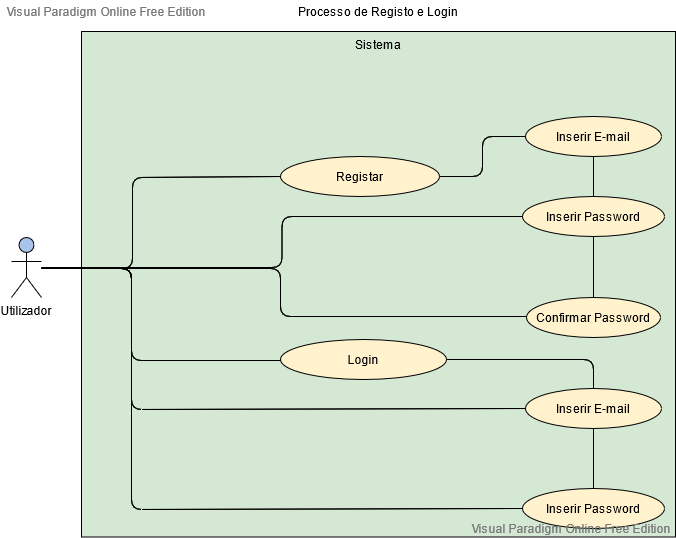
\includegraphics[scale=0.37]{loginsignup}	\caption[Diagrama de casos de uso: processo de registo e \emph{Login}]{Diagrama de casos de uso: processo de registo e \emph{Login}}
    \label{fig::casos-uso-regis}
\end{figure}

\begin{figure}[!htbp]
    \centering
    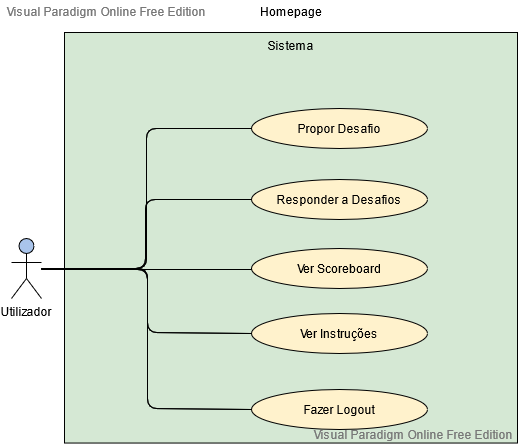
\includegraphics[scale=0.47]{homepage}
    \caption[Diagrama de casos de uso: \emph{homepage}]{Diagrama de casos de uso: \emph{homepage}.}
    \label{fig::casos-uso-homepage}
\end{figure}

\begin{figure}[!htbp]
    \centering
    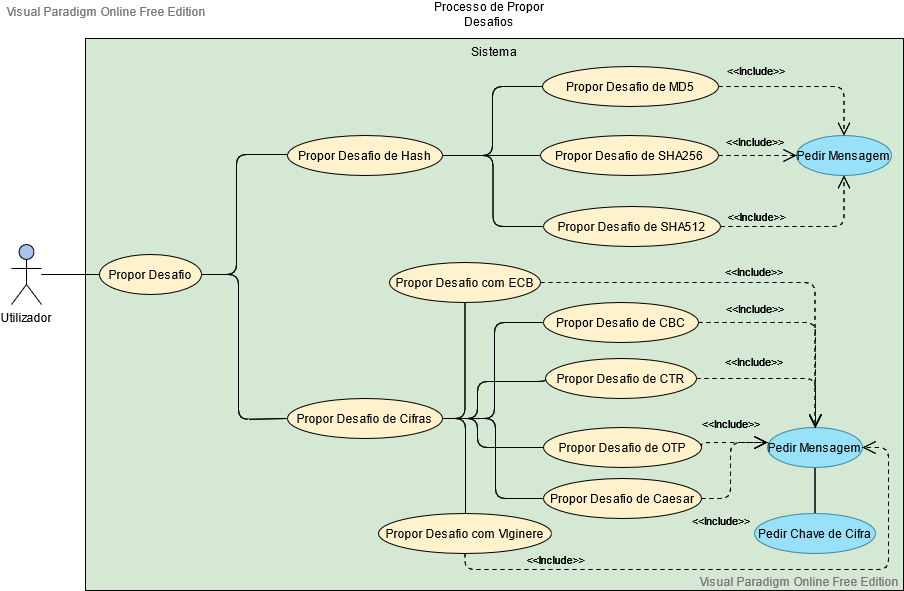
\includegraphics[scale=0.37]{addchallenge}
    \caption[Diagrama de casos de uso: processo de propor desafios]{Diagrama de casos de uso: processo de propor desafios.}
    \label{fig::casos-uso-propdesafio}
\end{figure}

\begin{figure}[!htbp]
    \centering
    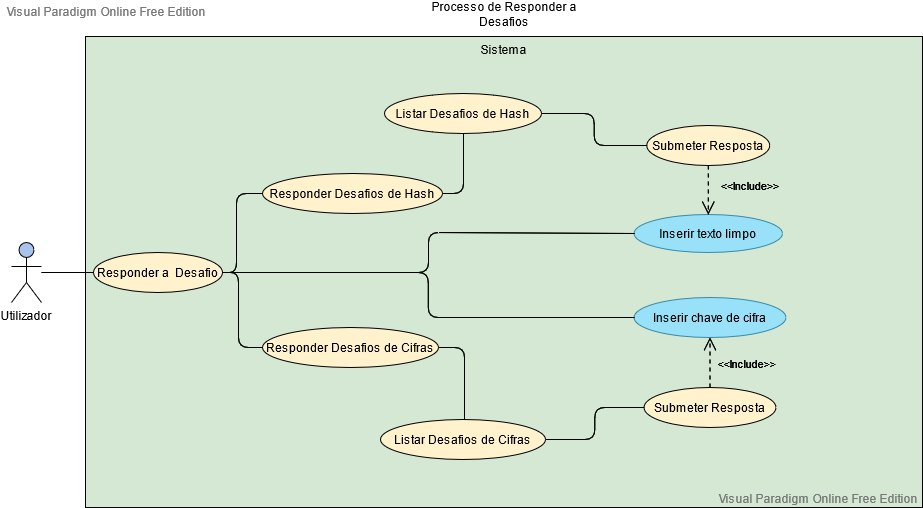
\includegraphics[scale=0.37]{solvechallange}
    \caption[Diagrama de casos de uso: processo de responder a desafios]{Diagrama de casos de uso: processo de responder a desafios.}
    \label{fig::casos-uso-repdesafio}
\end{figure}



\section{Modelo relacional da \acl{BD}}
\label{sec::engsoft:db}

É apresentada na Figura \ref{fig::diagrama-db} o modelo relacional da \acl{BD} delineada para o presente projeto.

\begin{figure}[!htbp]
    \centering
    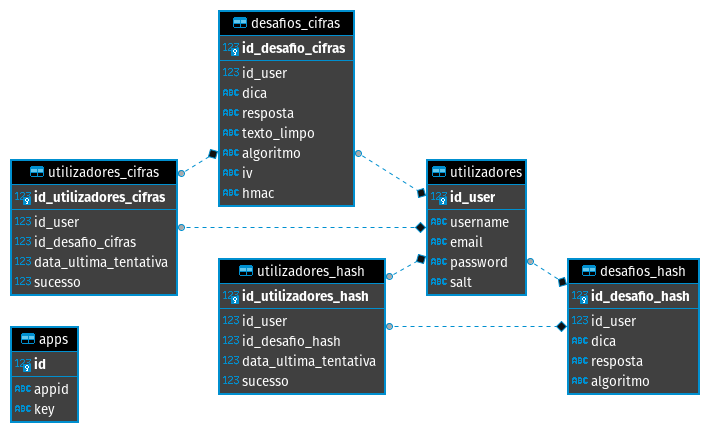
\includegraphics[width=\textwidth]{dbmodel}
    \caption[Modelo relacional]{Modelo relacional da \acl{BD}.}
    \label{fig::diagrama-db}
\end{figure}



\section{Arquitetura do sistema}
\label{sec::engsoft:arquitetura-sistema}

Uma vez que a base de dados é remota e o serviço prevê a utilização por vários utilizadores, é relevante separar a camada de \textbf{cliente} da camada de \textbf{servidor}. Tal implica que, por exemplo, o código da aplicação do cliente não contenha instruções de acesso direto à base de dados.

Desta forma, e a fim de agilizar o desenvolvimento e teste do serviço, o sistema foi concebido com a seguinte arquitetura (Figura \ref{fig::diagrama-sistema}):
\begin{itemize}
    \item \textbf{\acl{BD}} --- Alojada num servidor virtual \textit{Windows Server 2019};
    \item \textbf{\itshape Webservice} --- Alojado num servidor \textit{CentOS}, realiza a ponte entre o cliente e a base de dados, convertendo os pedidos do cliente em \textit{queries} para a \ac{BD};
    \item \textbf{Cliente} --- Aplicação local que comunica com o \textit{Webservice} por \ac{HTTPS}.
\end{itemize}

% A separação da \acl{BD} e do \textit{Webservice} permitiu realizar testes diretos com a base de dados enquanto o segundo era implementado.


\begin{figure}[!htbp]
    \centering
    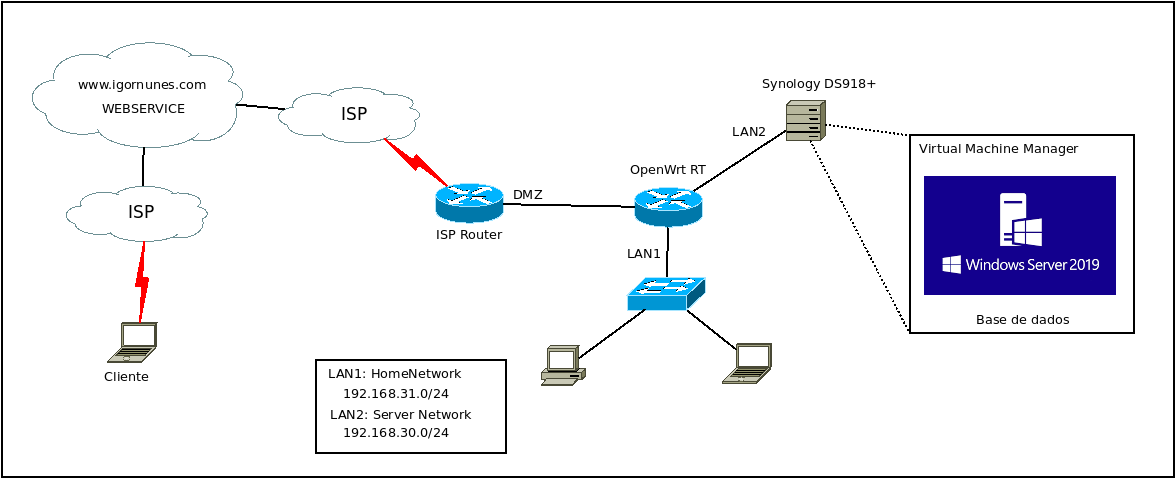
\includegraphics[width=\textwidth]{DiagramaActual}
    \caption[Diagrama da arquitetura do sistema]{Diagrama da arquitetura do sistema.}
    \label{fig::diagrama-sistema}
\end{figure}

%\begin{figure}[!htbp]
%    \centering
%    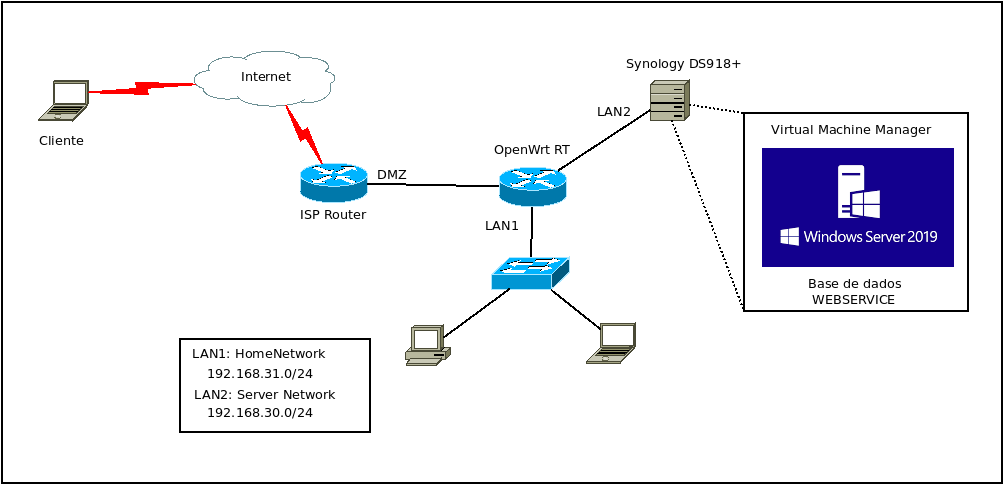
\includegraphics[scale=0.37]{DiagramaIdeal}	\caption[Diagrama da arquitetura do sistema]{Diagrama da arquitetura do sistema idealizada.}
%    \label{fig::diagrama-sistema}
%\end{figure}




\section{Conclusões}
\label{sec::engsoft:conclusao}

Na posse de um plano delineado segundo as práticas comuns da área da Engenharia de \textit{Software}, segue-se a fase de implementação, a qual deve seguir os requisitos determinados e tem por base os casos de uso estudados. Por fim, o sistema deverá seguir a arquitetura esquematizada.
